%% AMS-LaTeX Created with the Wolfram Language : www.wolfram.com

\documentclass[12pt]{article}
\usepackage{ceai} % Style file is in the project root.
\graphicspath{{../figs/}}

\begin{document}
\doublespacing	

\title{CE 488/5588: Applied AI for Engineering\\ \large Topic 3: ML Paradigms and Formalisms}
\author{}
\date{}
\maketitle

\section{Machine Learning: A Big-Picture View}
After surveying the scope of modern AI, we observe that the most robust and widely adopted arena of AI to date is \emph{data-enabled AI}, i.e., \emph{machine learning} (ML), including recent advances in deep learning and generative AI.

For most of the journey of this course, we will study this dominant paradigm of AI: \textbf{Machine Learning} (ML). Its reasoning structure aligns well with basic forms of human intelligence: ML is primarily \emph{inductive} during training (learning patterns from data) and primarily \emph{deductive} during inference (applying learned rules/parameters to new inputs).

In this topic, we focus on the learning (training) phase and attempt to answer two fundamental questions:

\begin{itemize}
\item How many machine learning types or \textit{paradigms} exist?
\item How to formulate the modeling in a machine learning paradigm or what are the basic learning \textit{formalisms}?
\end{itemize}

We state that there are three fundamental ML paradigms. Two of them are \emph{data-driven} (learning from a prepared dataset), while the third is \emph{interaction-driven} (data are generated through interaction with an environment):
\begin{itemize}
\item \textbf{Supervised Learning}
\item \textbf{Unsupervised Learning}
\item \textbf{Reinforcement Learning (RL)} (the agent generates training data through trial-and-error interaction rather than relying on a fixed, pre-collected dataset)
\end{itemize}
There are other ML types, including learning approaches between supervised and unsupervised learning (i.e., semi-supervised learning, weakly supervised learning), and self-supervised learning. Specifically, self-supervised learning stands as one of the frontiers of AI today. 

Regarding how to formulate a learning process—or, mathematically, how to represent the mapping between data, uncertainty, and decisions—we introduce two foundational learning formalisms:
\begin{itemize}
\item \textbf{Discriminative learning:} learn decision boundaries or conditional relations directly (e.g., $P(c\mid x)$ or a decision function $f(x)$).
\item \textbf{Generative learning:} learn a model of how data are generated (e.g., $p(x\mid c)$ and $P(c)$), which can then be used for inference via Bayes' rule.
\end{itemize}

During our ML journey, we will first focus on introducing \textit{Supervised Learning} and \textit{Unsupervised Learning}. We will start learning supervised learning theories and models. Unsupervised Learning will be introduced later after we have a solid understanding of Supervised Learning. For each, we will cover both discriminative and generative learning formalisms. Regarding RL, which is a unique learning paradigm and can be realized via discriminative or geneative learnign formalisms, will be briefly discussed. 


\section{Thought Experiment}

To make these ideas concrete, we use a drinking-water compliance thought experiment as an overarching example.

\begin{itemize}
\item Under \textbf{supervised learning}, we assume each sample has an observed outcome (a label), such as \textit{compliant/safe} vs. \textit{noncompliant/unsafe}.
\item In a \textbf{discriminative} approach, we learn a decision function that maps measurements (here, pH) directly to the label (e.g., learning $P(c\mid x)$ or a decision boundary).
\item In a \textbf{generative} approach, we instead model how the measurements are distributed within each class (e.g., learning $p(x\mid c)$ and $P(c)$), and then infer the most likely class using Bayes' rule.
\end{itemize}

The goal is not only to make a prediction, but to understand what each learning formalism assumes, what it learns from data, and how its limitations show up in practice.

\begin{ex-box}
\noindent \textbf{Drinking Water pH Compliance (Toy Example)}

An engineer monitors the safety/compliance of drinking water samples. One simple measured attribute is pH (potential hydrogen). She collects the following values for samples (say the total number of samples is \(N = 100\)):
\[
\bm{x} = \{7.8, 5.9, 9.0, 6.0, 7.8, \cdots \}
\]

The technical question arises: what technique or model should be used to decide whether a given sample is \textit{compliant/safe} or \textit{noncompliant/unsafe}?
\end{ex-box}

\section{Rule-based Decision Making and AI}
Before we dive deeper into ML, we briefly step back and ask: how might we make this decision \emph{classically}, without learning from data?

This perspective connects to \emph{symbolic AI} (also called \emph{rule-based AI} or ``good old-fashioned AI,'' GOFAI): knowledge is encoded explicitly as human-designed rules, and inference is primarily deductive.

Suppose the engineer adopts a simple rule based on a common drinking-water guideline: pH values in an acceptable range are generally considered compliant (often reported as approximately \(6.5\) to \(8.5\) in practice).

To simplify the discussion, we collapse the acceptable range into a single threshold at the upper bound and adopt the following rule as a decision function:
\[
  F(pH) = \left\{ 
    \begin{array}{ll}
      \mathrm{C0: compliant/safe} & \text{if } pH < 8.5, \\
      \mathrm{C1: noncompliant/unsafe} & \text{if } pH \geq 8.5.
    \end{array}
\right.
\]
This function shows that the value \(pH = 8.5\) is a threshold, or more formally, a decision boundary.

By applying this rule to the measured pH values, we see that the data point \(a_3 = 9.0\) will be evaluated as noncompliant/unsafe.

This rule-based decision-making process has always been a gold standard in engineering when making decisions (or in everyday decision-making). It is easy to imagine that early expert systems (another branch of AI) essentially adopted this paradigm for deductive inference before the late 1980s. 

\section{Supervised Learning: Classification}
There is a fundamental flaw in the rule-based decision-making process above. Even if it is valid under ideal assumptions, it can be far off in realistic scenarios.

Suppose an inspector (or laboratory test) provides outcomes for these samples based on an operational definition of compliance or safety. In this way, we obtain labeled data:
\[
\bm{c} = \{1, 1, 1, 0, 1, \cdots \}
\]
where 1 means \textit{compliant/safe} and 0 means \textit{noncompliant/unsafe}.

It is imperative for the engineer to recognize that the rule-based deductive approach should be revised in favor of letting the data speak. She therefore adopts an ML process. To proceed, she illustrates the data as follows:
\begin{figure} [ht]
         \centering
         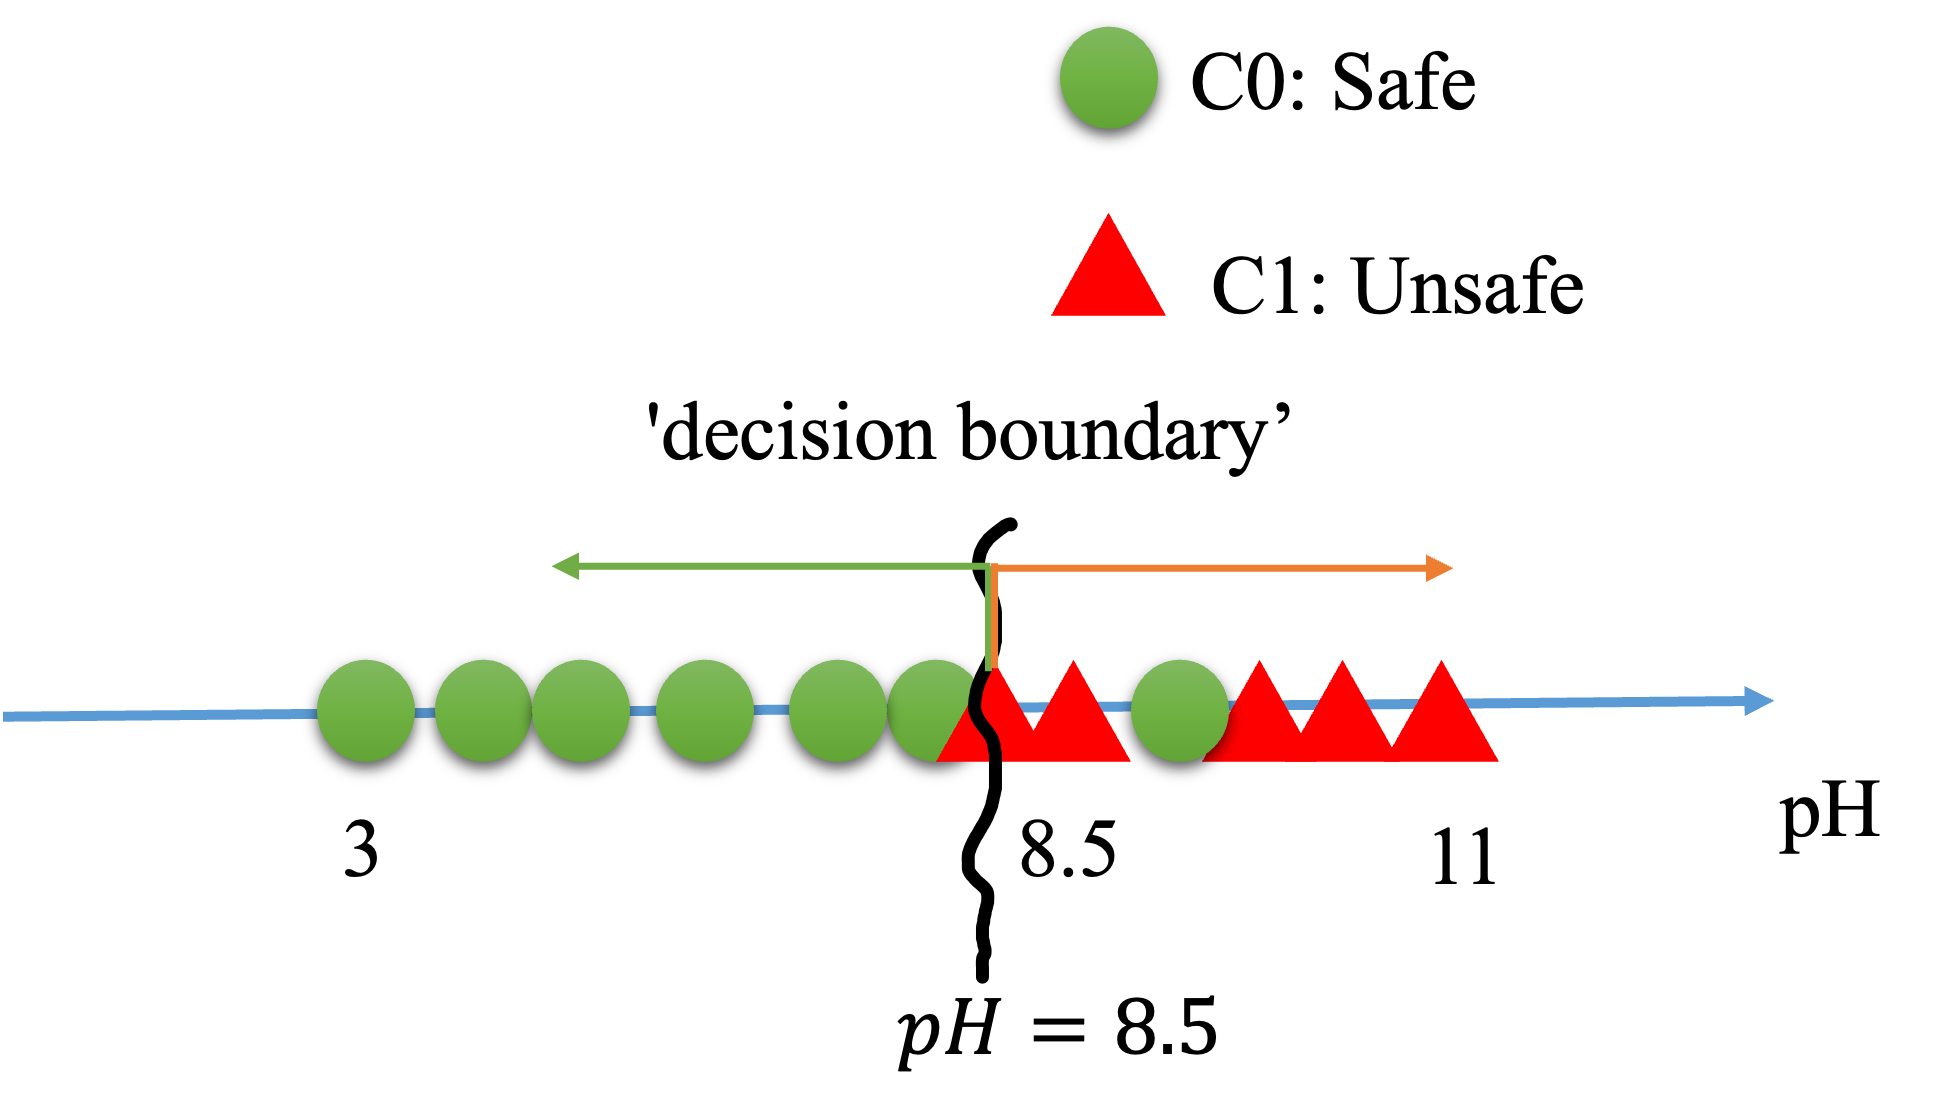
\includegraphics[width=0.6\textwidth]{../figs/pHvalues_2.png}
        \caption{Drinking-water pH measurements with a guessed decision boundary.}
        \label{pHvalues}
\end{figure}

The engineer observes that the simple rule may not match observed outcomes. While \(pH = 8.5\) is a convenient threshold for illustration, the effective decision boundary could shift depending on the specific operational definition of compliance, measurement uncertainty, and other covariates. What is an objective approach for resolving such disagreements?

At this moment, we state that this toy example provides a meaningful instance for applying supervised machine learning, which in this case, is \textit{supervised classification}.

To sum up, the data sets we have are:
\[
\bm{x} = \{7.8, 5.9, 9.0, 6.0, 7.8, \cdots \} 
\]
\[
\bm{c} = \{1, 1, 1, 0, 1, \cdots \}
\]
The two vectors can be more formally defined as:
\begin{equation}
\bm{D} = \{ (x_i, c_i) \mid x_i \in [0, 10],\, c_i \in \{0, 1\},\, i = 1, 2, \cdots, N \}
\label{lec03eq01}
\end{equation}
which is a labeled data set, and \(x_i\) is an instance of measurement (or feature, if extracted from a raw data set) and \(c_i\) is an instance of labeling.  

Given the dataset above, the engineer's task is to devise a machine learning model that can classify a given measurement (i.e., a pH value) into two categories: \(c = 1\) means \textit{compliant/safe} and \(c = 0\) means \textit{noncompliant/unsafe}.

More formally, a supervised model is defined by learning from a labeled dataset (Eq.~\ref{lec03eq01}), mapping a measurement (or feature) variable \(x\) to a label variable \(c\). A generic binary classifier can be written as:
\begin{equation}
m(x \mid \bm{w}) = \left\{ 
    \begin{array}{ll}
      c_1 & \text{if } f(x \mid \bm{w}) \geq \sigma,  \\
      c_0 & \text{if } f(x \mid \bm{w}) < \sigma,
    \end{array}
\right.
\label{lec03eq02}
\end{equation}
where \(\bm{w}\) is the model parameter vector used in the decision function \(f(x \mid \bm{w})\). The equation \(f(x \mid \bm{w}) - \sigma = 0\) (equivalently \(f(x \mid \bm{w}) = \sigma\)) defines a decision boundary in the feature space.

In the earlier rule-based case, we effectively had \(f(x \mid \bm{w}) = x\) with \(\sigma = 8.5\). In general, \(f\) can be nonlinear, and \(\sigma\) can be treated as an additional model parameter (or absorbed into \(\bm{w}\) by augmenting the feature vector).

For the sake of simplicity, the classification model in Eq.~\ref{lec03eq02} is binary (with two class labels, \(c_0\) and \(c_1\)). In practice, classification can be multi-class (more than two class labels exist). Fig.~\ref{pHvalues_2} illustrates the resulting classification based on the decision function \(f(x \mid \bm{w})\). In other words, the classification is now conducted in a transformed feature (or decision-variable) space of \(f(x)\).

\begin{figure} [ht]
         \centering
         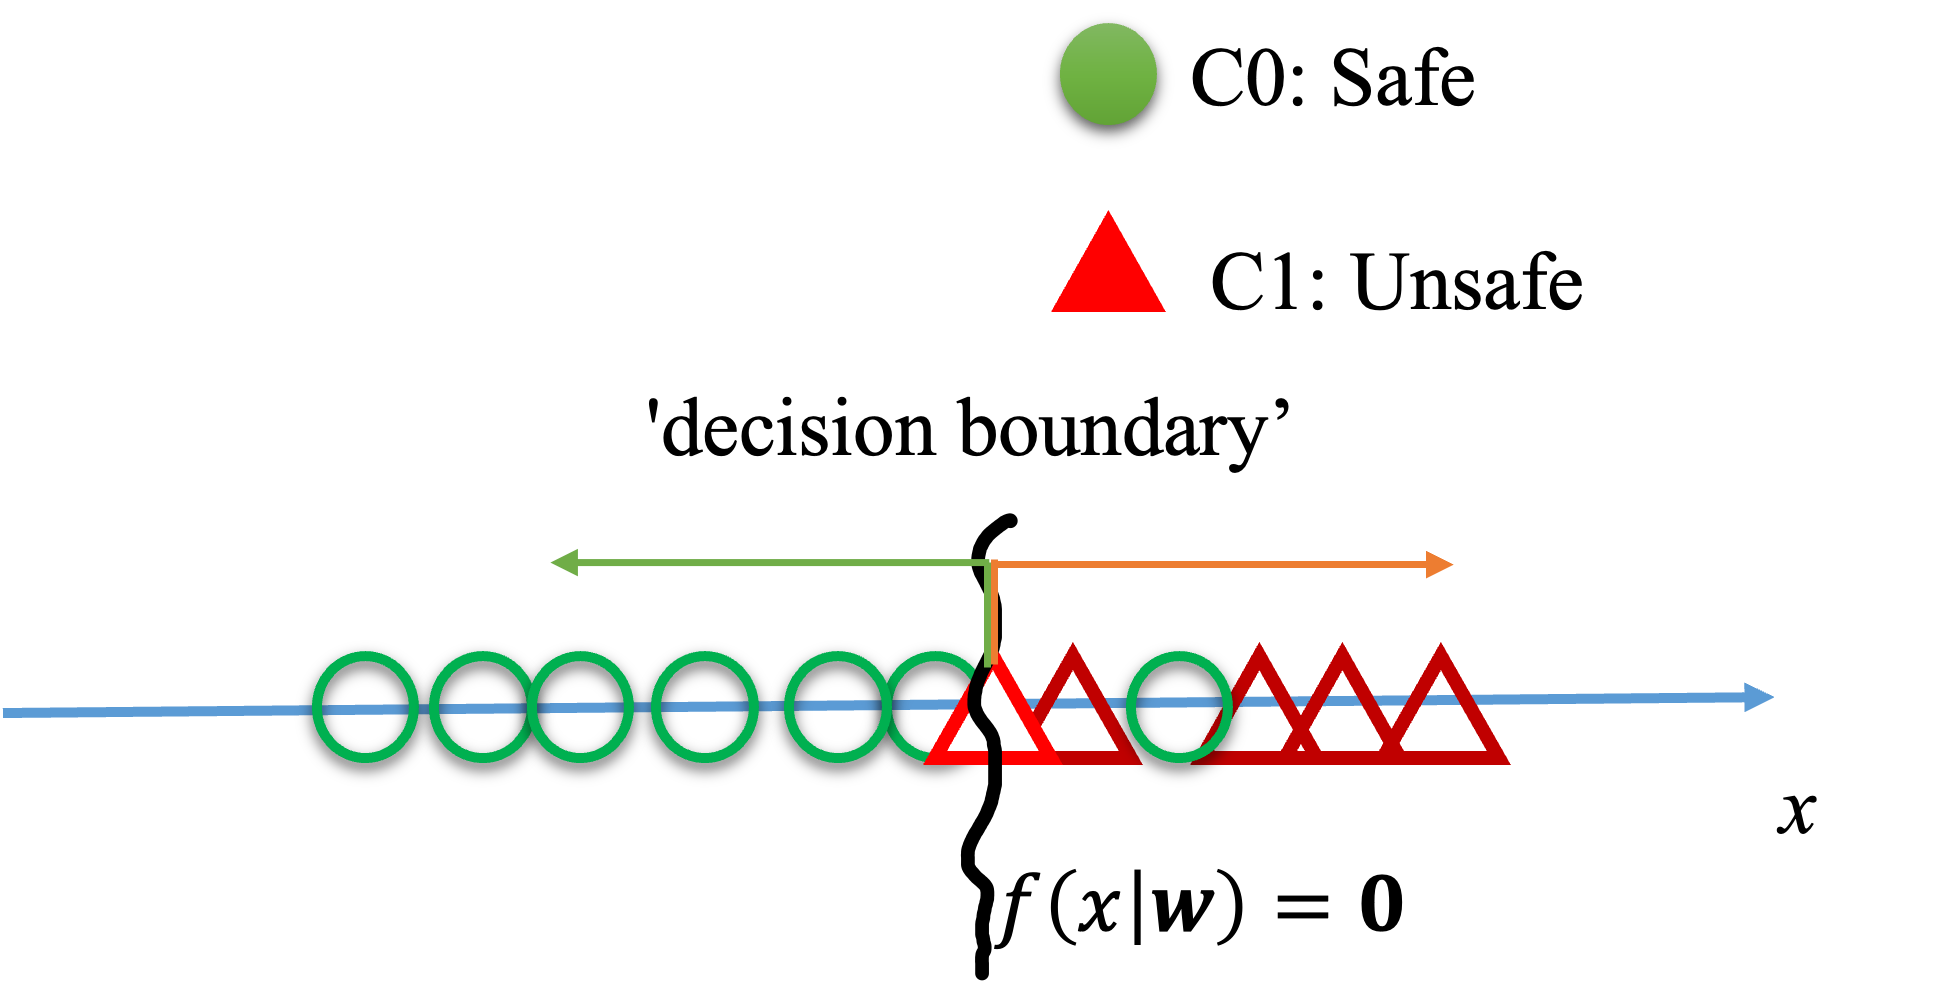
\includegraphics[width=0.6\textwidth]{../figs/pHvalues_transformed_2.png}
        \caption{Classification in a transformed space of \(f(x \mid \bm{w})\).}
        \label{pHvalues_2}
\end{figure}

With the explanation above, we can recognize that there is no need to express a function for the predictive ML model \(m(x \mid \bm{w})\) separately; it is the decision function \(f(x \mid \bm{w})\) that matters. If we include multi-class labels, a decision function can be transformed in a way such that inferring a class label \(c\) is based on the following optimization scheme:
\begin{equation}
    c^* = \mathrm{argmax}_c\, f(x \mid \bm{w})
    \label{eq:infer}
\end{equation}
This means that the predicted class label \(c^*\) is the one that maximizes the decision function given an input \(x\). In ML practice, the numeric value of \(f(x \mid \bm{w})\) given an input \(x\) can be called a score. 

There are two learning formalisms to realize this learning process: Discriminative Learning and Generative Learning.

\section{Discriminative Learning}
\subsection{Formulation}
Discriminative Learning is a formalism that directly constructs a decision function using a predefined function structure and a set of parameters; subsequently, these parameters are learned from a data set via an optimization-based parameter estimation process. 

For the supervised learning (classification) problem above, the data is labeled. To learn the decision function weights from data, a loss function is often defined so that a wrong prediction (given an input \(x\)) is penalized. The total loss, as a function of the parameter vector \(\bm{w}\), is minimized through an optimization process.

In upcoming lectures, we will go through several classic supervised, discriminative classification models, including (1) logistic regression (parametric); (2) feed-forward neural networks (parametric); and (3) support vector machines (non-parametric).

To this end, if the input (measurement or feature) variable \(x\) is a scalar, one may simply consider it directly. Returning to the original water quality assessemnt task, the engineer might use another physical measure, for example, the PFAS level ($y$, part per millions, or PPP) (\(\%\)) to better characterize water quality. A more reasonable representation of the underlying water quality should use a vector, namely \(\bm{x} = [x; y]\), where \(x\) is the pH value and \(y\) is the PPP value. The decision boundary must then be illustrated in a 2-D Euclidean space. 

\begin{figure} [ht]
         \centering
         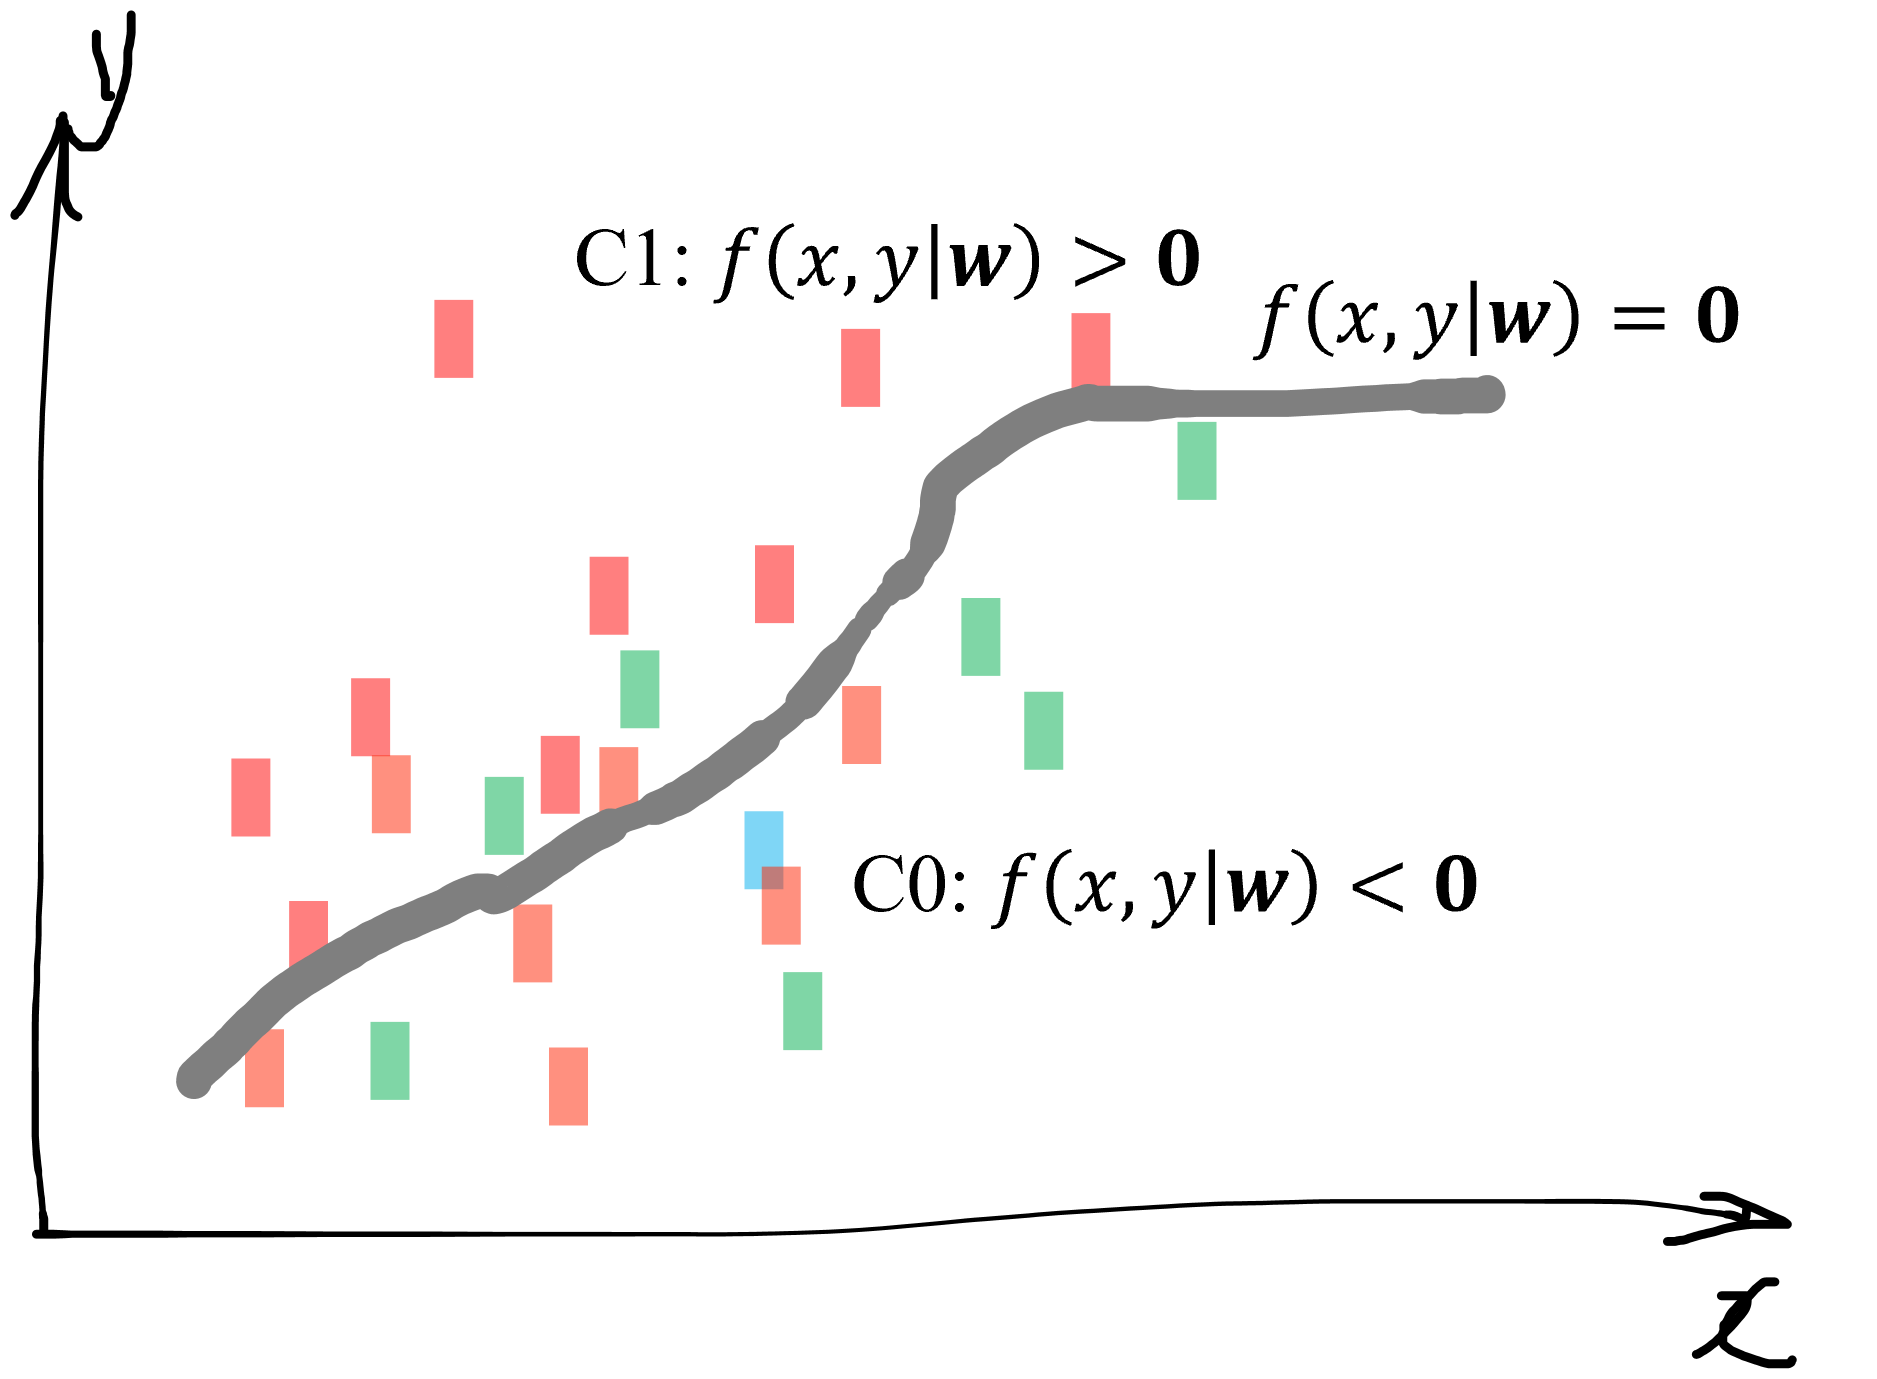
\includegraphics[width=0.4\textwidth]{../figs/nl_boundary.png}
        \caption{Nonlinear decision boundary defined by \(f(x,y \mid \bm{w})\) (more generally, for a feature vector \(\bm{x}\), the decision boundary \(f(\bm{x} \mid \bm{w})\) can be highly nonlinear and complex).}
        \label{nl_boundary}
\end{figure}

Given an implicitly defined decision function $f(x,y\mid\bm{w})=0$, the resulting decision boundary in the $x$--$y$ plane can be nonlinear. More generally, when high-dimensional feature vectors are used for classification, the decision function may define a highly nonlinear (and potentially complex) surface in feature space. Estimating the parameters $\bm{w}$ can then become substantially more difficult due to the \emph{curse of dimensionality}\footnote{See the Wikipedia article \emph{``Curse of dimensionality''} for an overview of how the volume of high-dimensional spaces grows rapidly and why this can degrade learning, density estimation, and nearest-neighbor reasoning.}. Many treatments exist to address this, with classic approaches including non-parametric modeling using kernel methods.

\subsection{Decision Function Modeling}
To learn an ML model—equivalently, to estimate the model parameters based on the labeled data—there are two types of modeling methods: Parametric vs. Non-parametric Modeling.

The configuration of the parameter set \(\bm{w}\) in the decision function \(f(x \mid \bm{w})\) leads to two modeling structures:
\begin{itemize}
\item \textbf{Parametric models:} The dimension of \(\bm{w}\) is fixed and does not depend on the number of data points in \(\bm{D}\). Learning models in this category include logistic regression, neural networks, and even deep neural networks.
\item \textbf{Non-parametric models:} The effective complexity of the model can grow with the number of data points (e.g., via support vectors in SVMs or kernel methods). Here, the decision function is often expressed as \(f(x \mid \bm{w}, \bm{D})\), explicitly incorporating the labeled dataset \(\bm{D}\).
\end{itemize}

\subsection{Toy Example}
In this toy example, we simulate some data and implement two ML approaches: (1) rule-based classification by choosing a threshold (i.e., \(pH = 8.5\)); and (2) discriminative classification using a linear function \(f(x) = w_0 + w_1 x\). Note that for the linear model we do not learn the parameters from data but instead set them directly for illustration. To simplify, we assume that 16 pH values (all integers) are collected. To verify the effectiveness of the two models, we calculate the classification error.

Taking one example dataset:
\[
\text{pH} = \{7, 7, 6, 2, 2, 14, 8, 5, 7, 1, 14, 1, 1, 1, 9, 4\}
\]
\[
\text{Label} = \{G, G, G, G, G,  B, G, G,  B, G,  B, G, G, G, G, G\}
\]

Using the rule-based classification, we obtain the following confusion matrix:
\[
\begin{array}{cc|c|c|}
    & \multicolumn{1}{c}{} & \multicolumn{2}{c}{\text{Predicted}} \\
    & \multicolumn{1}{c}{} & \text{Good} & \text{Bad} \\ \cline{3-4}
    \multirow{2}{*}{\rotatebox[origin=c]{90}{\text{Actual}}} & \text{Good} & 12 & 1 \\ \cline{3-4}
    & \text{Bad} & 1 & 2 \\ \cline{3-4}
\end{array}
\]
The overall accuracy of this model is:
\[
\text{OA} = \frac{12+2}{16} = 87.5\%
\]

Using a linear discriminative function \(f(x) = -8 + 2x\) for classification yields the confusion matrix:
\[
\begin{array}{cc|c|c|}
    & \multicolumn{1}{c}{} & \text{Good} & \text{Bad} \\ \cline{3-4}
    \multirow{2}{*}{\rotatebox[origin=c]{90}{\text{Actual}}} & \text{Good} & 6 & 7 \\ \cline{3-4}
    & \text{Bad} & 0 & 3 \\ \cline{3-4}
\end{array}
\]
The overall accuracy of this model is:
\[
\text{OA} = \frac{6+3}{16} = 56.3\%
\]
This implies that the arbitrarily set linear-function model provides a worse prediction compared to the rule-based model. (Note that in practice, the linear model parameters would be optimized based on the data.)

\section{Generative Learning}
\subsection{Formulation}
In discriminative learning, the decision function is directly parameterized and learned from data. In contrast, generative learning seeks to model how the data (features/measurements) are generated with respect to the underlying classes. 

This approach assumes that there is a model describing how data points are generated. ML does not concern itself with the physical data-generation process; instead, we use a probability distribution.

The starting point is to plot the histogram of the measurements, which provides an initial impression of the data distribution (see Fig.~\ref{hist_bayes}(a)).

\begin{figure}[ht]
    \centering
    \begin{subfigure}[b]{0.45\textwidth}
        \centering
        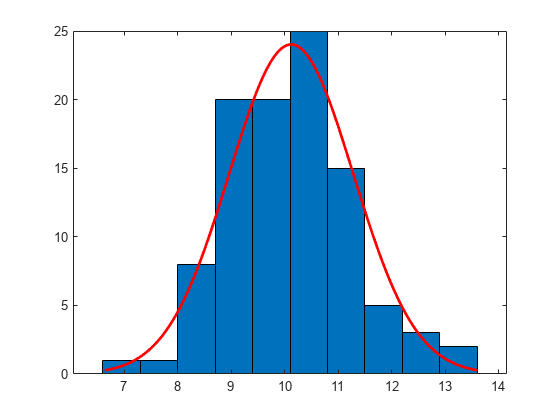
\includegraphics[width=\textwidth]{histo_distri.png}
        \caption{Histogram of measurements.}
    \end{subfigure}
    \hfill
    \begin{subfigure}[b]{0.45\textwidth}
        \centering
        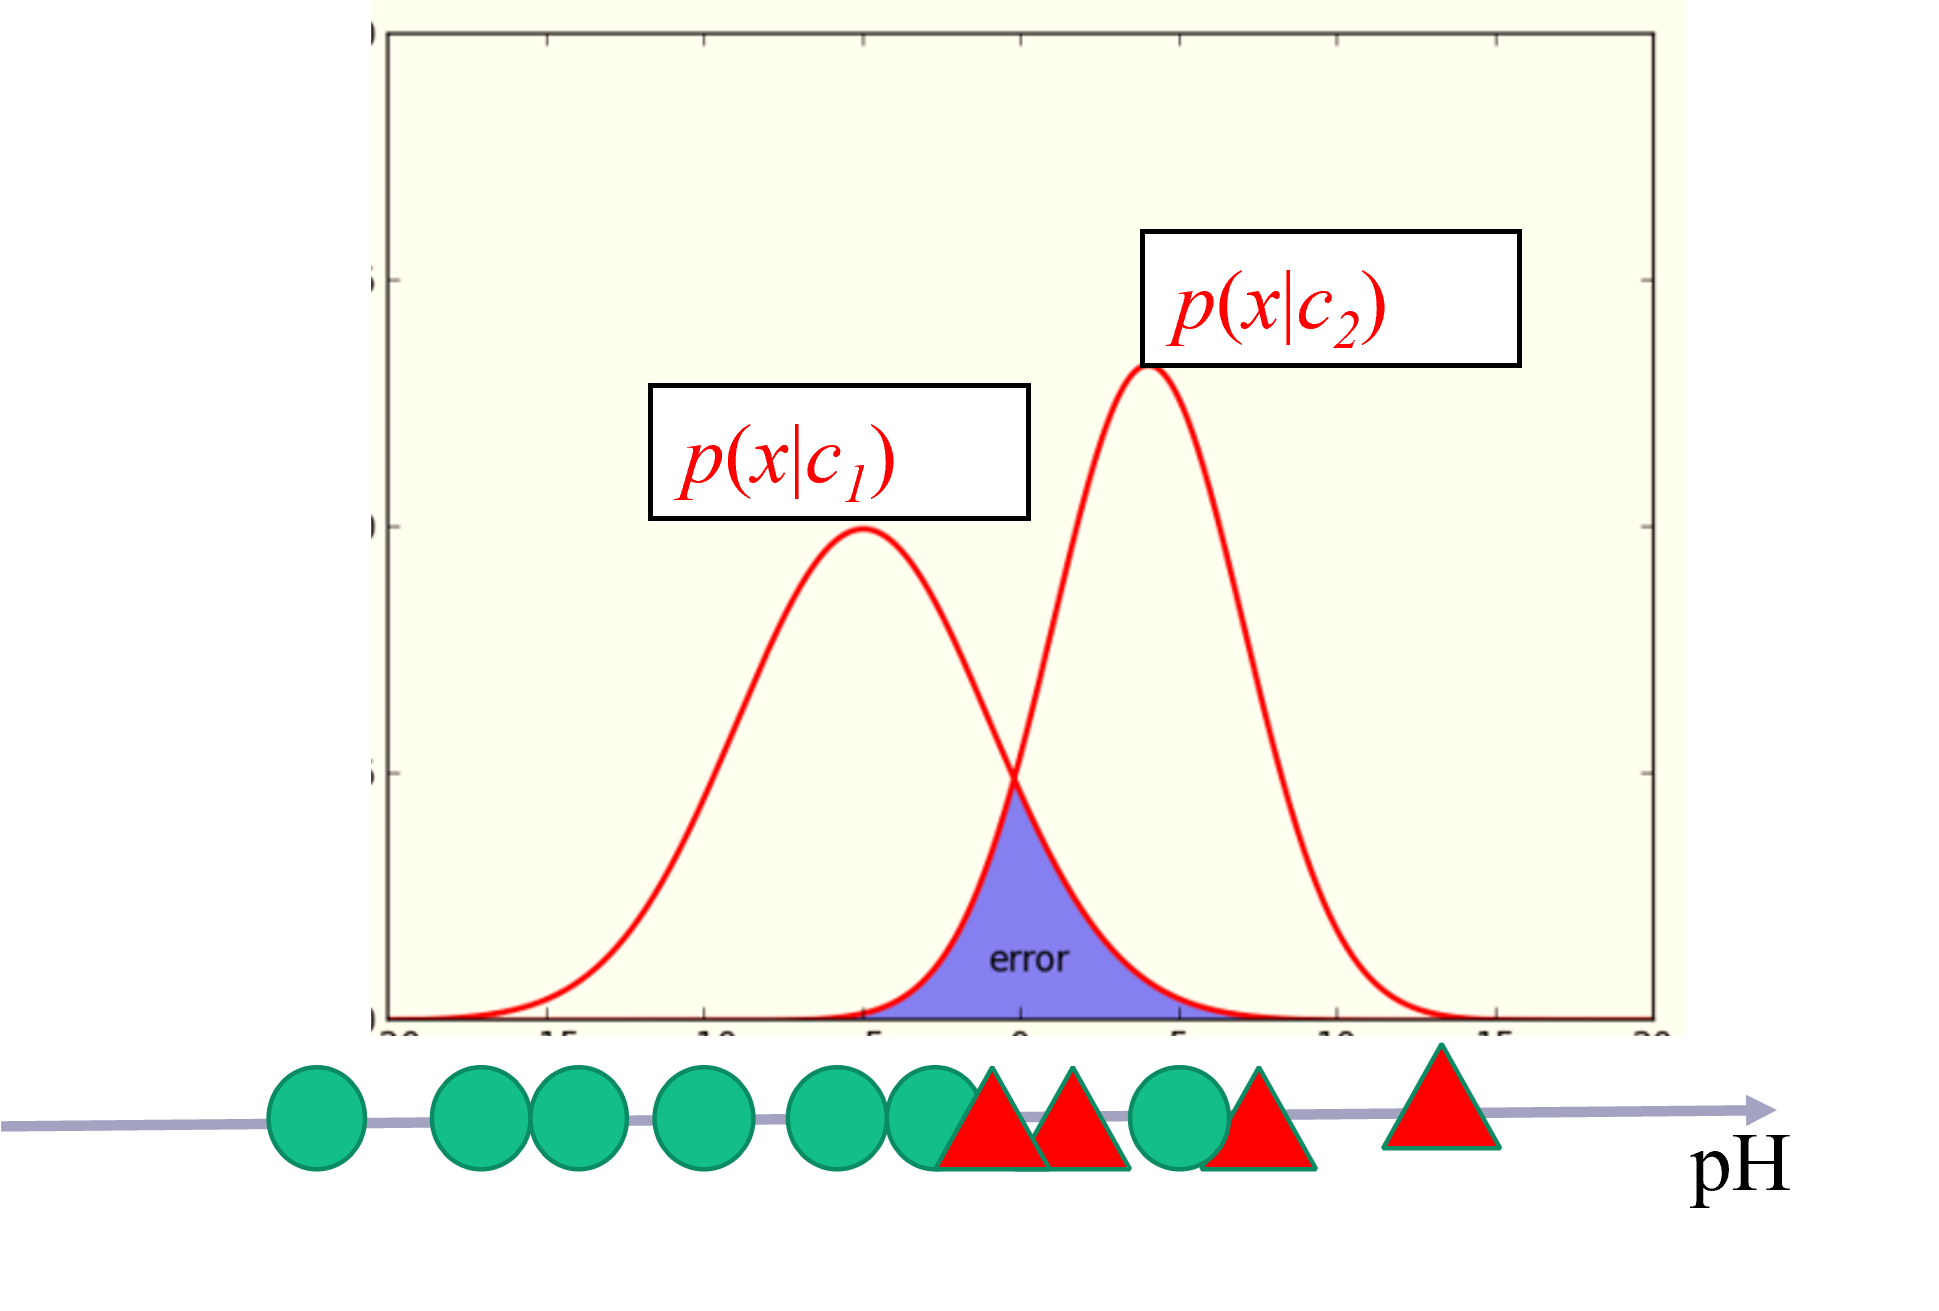
\includegraphics[width=\textwidth]{bayes.png}
        \caption{Class-conditional densities (illustration).}
    \end{subfigure}
    \caption{Histogram and illustrative class-conditional distributions used in generative learning.}
    \label{hist_bayes}
\end{figure}

Standard probability models include Gaussian (Normal) distributions, exponential family models, and others. Statistical techniques estimate a probability density function (PDF) for data that belongs to a class. In general, we define a probability function conditional on a class variable \(c\) as \(p(x \mid c)\). In Fig.~\ref{hist_bayes}(b), two density functions illustrate the distribution of the pH variable, conditional on the class labels \(c_1\) and \(c_2\), respectively. Note that any PDF must satisfy:
\[
\int_{-\infty}^{\infty} p(x \mid c) \, \mathrm{d}x = 1.
\]

Second, while the measurements \(x\) are continuous, the labels \(c\) are categorical, so we use a probability mass function (PMF) \(P(c)\) which satisfies:
\[
\sum_{c} P(c) = 1.
\]
For binary labeling, \(P(c = 1) + P(c = 0) = 1\).

Using Bayes' theorem, the generative model is given by:
\begin{equation}
\begin{split}
P(c \mid x) &= \frac{P(x, c)}{p(x)} \\
           &= \frac{p(x \mid c)P(c)}{p(x)}.
\end{split}
\label{bayes01}
\end{equation}
Here,
\begin{itemize}
\item \(p(x \mid c)\) is the likelihood function (or the PDF of \(x\) given \(c\)).
\item \(P(c)\) is the prior probability (or the PMF of \(c\)).
\item \(P(x, c)\) is the joint distribution of \(x\) and \(c\).
\item \(P(c \mid x)\) is the posterior probability.
\item \(p(x)\) is the marginal PDF of \(x\).
\end{itemize}

Since \(p(x)\) is independent of \(c\), it can be treated as a normalization constant, leading to the proportionality:
\begin{equation}
    P(c \mid x) \propto p(x \mid c)P(c).
    \label{bayes02}
\end{equation}

Thus, the prediction is made as:
\[
c^* = \mathrm{argmax}_c\, p(x \mid c)P(c).
\]

\subsection{Toy Example: Coin Tossing (Discrete Measurements)}
Up to this point, our running example used a continuous measurement (pH). A natural next step in generative learning would be to model $p(x\mid c)$ with a continuous density such as a Gaussian.

However, introducing continuous probability densities and Gaussian modeling can add unnecessary overhead at this stage. To keep the focus on Bayes' rule and the idea of modeling $p(x\mid c)$, we first use a simpler \emph{discrete} toy example.

\paragraph{Setup.}
Consider a classification problem with two classes, $c\in\{H, T\}$, and a binary-valued measurement $x\in\{-1, 1\}$.

You can interpret $x$ as the outcome of a coin toss encoded as
\begin{itemize}
    \item $x=1$ for \textit{Heads},
    \item $x=-1$ for \textit{Tails}.
\end{itemize}

An experiment collects 1000 labeled observations, and the class priors are estimated by counting:
\begin{align*}
P(H) &= \frac{\#\,H}{1000} = 0.8, \\
P(T) &= \frac{\#\,T}{1000} = 0.2.
\end{align*}

The conditional probability mass functions for $x$ given the classes are estimated as:
\begin{align*}
P(x=-1 \mid H) &= \frac{\#(x=-1)}{\#\,H} = 0.7, \quad & P(x=1 \mid H) &= \frac{\#(x=1)}{\#\,H} = 0.3, \\
P(x=-1 \mid T) &= \frac{\#(x=-1)}{\#\,T} = 0.2, \quad & P(x=1 \mid T) &= \frac{\#(x=1)}{\#\,T} = 0.8.
\end{align*}

\paragraph{Inference.}
To classify a new observation $x$, we compute posterior probabilities using Bayes' theorem. For an observation $x=1$:
\begin{align*}
P(x=1) &= P(x=1 \mid H)P(H) + P(x=1 \mid T)P(T) \\
       &= 0.3 \times 0.8 + 0.8 \times 0.2 \\
       &= 0.4.
\end{align*}
Then, the posterior probabilities are:
\begin{align*}
P(H \mid x=1) &= \frac{0.3 \times 0.8}{0.4} = 0.6, \\
P(T \mid x=1) &= \frac{0.8 \times 0.2}{0.4} = 0.4.
\end{align*}

Given $x=1$, the model classifies the observation as belonging to class $H$ because $P(H\mid x=1) > P(T\mid x=1)$.

\subsection{Generative learning vs. generative AI}
At this point, it is useful to distinguish \emph{generative learning} (as introduced in this topic) from modern \emph{generative AI}.

\paragraph{Generative learning (classical viewpoint).}
In classical ML, \emph{generative learning} typically means fitting an explicit probabilistic model for the data-generating process (e.g., estimating $p(x\mid c)$ and $P(c)$ for classification). Such models support uncertainty-aware inference (via Bayes' rule) and often have relatively transparent assumptions.

\paragraph{Generative AI (modern viewpoint).}
Modern \emph{generative AI} usually refers to \emph{foundation-scale} neural generative models---such as large language models and diffusion models---that learn high-dimensional data distributions and can synthesize text, images, audio, or code.

A key difference is the \textbf{learning complexity}. Generative AI models are typically trained in multiple stages:
\begin{itemize}
\item \textbf{Self-supervised pretraining} on massive datasets to learn rich representations and a generative objective (e.g., next-token prediction for LLMs or denoising/noise-prediction for diffusion models).
\item \textbf{Task adaptation} (often supervised fine-tuning / instruction tuning) to align the generator with downstream tasks and human intent.
\item \textbf{Preference optimization} (often reinforcement learning from human feedback or related methods) to improve usefulness, safety, and adherence to constraints.
\end{itemize}

While all these stages can influence behavior, the core ``generative power'' largely comes from large-scale representation learning during self-supervised pretraining.


\section{Conclusion Remarks}
This topic established a high-level map of machine learning as the dominant, data-enabled paradigm of modern AI. We introduced three core ML paradigms—supervised learning, unsupervised learning, and reinforcement learning—and emphasized how ML combines \emph{inductive} learning during training with largely \emph{deductive} computation during inference.

Using a drinking-water pH compliance scenario as a running example, we contrasted two foundational learning formalisms for supervised classification:
\begin{itemize}
\item \textbf{Discriminative learning}, which learns decision boundaries or $P(c\mid x)$ directly.
\item \textbf{Generative learning}, which models how data are generated (e.g., $p(x\mid c)$ and $P(c)$) and performs inference via Bayes' rule.
\end{itemize}

We also used a discrete coin-toss toy example to illustrate Bayesian generative classification without requiring continuous density models, and we clarified how classical generative learning relates to (but differs from) modern generative AI systems.

In subsequent topics, we will develop concrete discriminative models (e.g., logistic regression, neural networks, and SVMs), discuss optimization and generalization, and connect these classical foundations to modern deep and generative models.

\end{document}
